%===========================================
\chapter{Décomposer le problème}
\index{décomposer le code}
%===========================================

%===================
\section{Motivation}
%===================

	Jusqu’à présent, 
	les problèmes que nous avons abordés étaient relativement petits.
	Nous avons pu les résoudre avec un algorithme d’un seul tenant.
	
	Dans la réalité,
	les problèmes sont plus gros 
	et il devient nécessaire de les décomposer en sous-problèmes.
	On parle d’une \emph{approche modulaire}.
	Les avantages d’une telle décomposition sont multiples.
	\begin{itemize}
	\item
		\textbf{Cela permet de libérer l’esprit.}
		L’esprit humain ne peut pas traiter trop d’informations à la fois
		(\emph{surcharge cognitive}).
		Lorsqu’un sous-problème est résolu,
		on peut se libérer l’esprit et attaquer un autre sous-problème.
	\item
		\textbf{On peut réutiliser ce qui a été fait.}
		Si un même sous-problème apparait plusieurs fois
		dans un problème ou à travers plusieurs problèmes,
		il est plus efficace de le résoudre une fois et
		de réutiliser la solution.
	\item
		\textbf{On accroit la lisibilité.}
		Si, dans un algorithme, 
		on appelle un autre algorithme pour résoudre un sous-problème,
		le lecteur verra un nom d’algorithme qui peut être plus parlant
		que les instructions qui se cachent derrière, même s’il y en a peu.
		Par exemple, \lda{dizaine(nb)} est plus parlant que
		\lda{nb MOD 100 DIV 10} pour calculer les dizaines d’un nombre.
	\end{itemize}

	Parmis les autres avantages, 
	que vous pourrez moins percevoir en début d’apprentissage,
	citons la possibilité de répartir le travail dans une équipe.
	
	Un algorithme qui résout une partie de problème
	est parfois appelé \textbf{fonction}\index{fonction}, 
	\textbf{procédure}\index{procédure}, 
	\textbf{méthode}\index{méthode} ou encore
	\textbf{module}\index{module}
	en fonction du langage et du contexte.
	Il y a quelques nuances mais elles importent peu ici.
	
%===================
\section{Exemple}
%===================

	Illustrons l’approche modulaire sur 
	le calcul du maximum de 3 nombres.

	\begin{center}
	\flowalgoddd{a (réel)}{b (réel)}{c (réel)}{max3}{réel}
	\end{center}
	
	Commençons par écrire la solution du problème plus simple~:~
	le maximum de 2 nombres.

	\begin{minipage}{6cm}
		\flowalgodd{a (réel)}{b (réel)}{max2}{réel}
	\end{minipage}
	\quad
	\begin{minipage}{7cm}
		\begin{LDA}
		\Algo{max2}{\Par{a}{réel}, \Par{b}{réel}}{réel}
			\Decl{max}{réel}
			\If{a > b}
				\Let max \Gets a
			\Else
				\Let max \Gets b
			\EndIf
			\Return max
		\EndAlgo
		\end{LDA}
	\end{minipage}
	
	Pour le maximum de 3 nombres, il existe plusieurs approches.
	Voyons celle-ci~:

	\begin{LDA}
		\Stmt 1) Calculer le maximum des deux premiers nombres, soit \lda{maxab}
		\Stmt 2) Calculer le maximum de \lda{maxab} et du troisième nombre, ce qui donne le résultat.
	\end{LDA}

	qu’on peut illustrer ainsi~:
	
	\begin{center}
	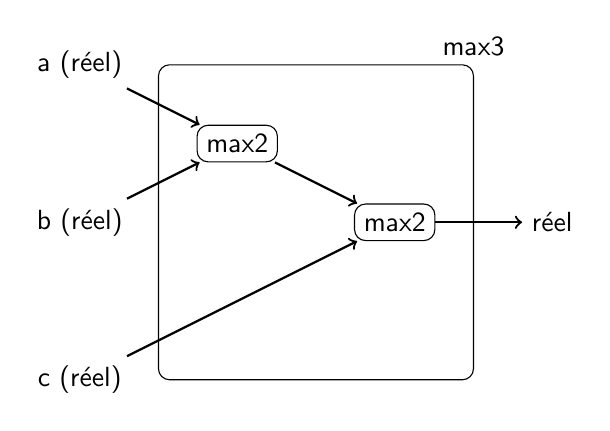
\begin{tikzpicture}[auto]
		\sffamily
		\node (a) at (0,4) {a (réel)};
		\node (b) at (0,2) {b (réel)};
		\node (c) at (0,0) {c (réel)};
		\node[draw,rounded corners] (max2a) at (2,3) {max2};
		\node[draw,rounded corners] (max2b) at (4,2) {max2};
		\node (r) at (6,2) {réel};
		\draw[rounded corners] (1,0) rectangle (5,4) node[above] {max3};
		\draw[->,thick] (a) to (max2a);
		\draw[->,thick] (b) to (max2a);
		\draw[->,thick] (c) to (max2b);
		\draw[->,thick] (max2a) to (max2b);
		\draw[->,thick] (max2b) to (r);
	\end{tikzpicture}	
	\end{center}
	
	Sur base de cette idée, 
	on voit que calculer le maximum de trois nombres
	peut se faire en calculant deux fois le maximum de deux nombres.
	On ne va évidemment pas \emph{recopier}%
	\footnote{
		Cette approche serait fastidieuse,
		engendrerait de nombreuses erreurs lors du recopiage
		et serait difficile à lire.
	} dans notre solution
	ce qu’on a écrit pour le maximum de deux nombres~;
	on va plutôt y faire référence, 
	c’est-à-dire appeler l’algorithme \lda{max2}. 
	Ce qui donne~:

	\begin{LDA}
	\Algo{max3}{\Par{a}{réel}, \Par{b}{réel}, \Par{c}{réel}}{réel}
		\Decl{maxab, max}{réels}
		\Let maxab \Gets max2(a,b)
		\Let max \Gets max2(maxab,c)
		\Return max
	\EndAlgo
	\end{LDA}

	qu’on peut encore simplifier en~:
	
	\begin{LDA}
	\Algo{max3}{\Par{a,b,c}{réels}}{réel}
		\Return max2( max2(a,b) ,c)
	\EndAlgo
	\end{LDA}

%===================
\section{Les paramètres}
\index{paramètres}
%=======================

	Jusqu’à présent,
	nous avons considéré que les paramètres d’un algorithme (ou \emph{module}\index{module})
	correspondent à ses données et que le résultat, unique,
	est retourné.

	Il s’agit d’une situation fréquente mais pas obligatoire
	que nous pouvons généraliser.
	En pratique, on peut rencontrer trois sortes de paramètres.

	%==================================
	\subsection{Le paramètre en entrée}
	%==================================

		Le paramètre en \textbf{entrée}
		est ce que nous connaissons déjà.
		Il correspond à une donnée de l’algorithme.
		Une valeur va lui être attribuée en début d’algorithme
		et elle ne sera pas modifiée.
		On pourra faire suivre le nom du paramètre d’une flèche
		vers le bas (\In) pour rappeler son rôle.
		
		Lors de l’appel, on fournit la \textbf{valeur}
		ou, plus généralement une expression
		dont la valeur sera donnée au paramètre.
		Voici un cas général de paramètre en entrée.
		
		\begin{minipage}{4cm}
			\begin{LDA}
				\LComment {Code appelant}
				\Stmt monAlgo(expr)
				\Empty
			\end{LDA}
		\end{minipage}
		\quad
		\begin{minipage}{8cm}
			\begin{LDA}
				\LComment {Code appelé}
				\Entete{monAlgo}{\Par{par\In}{entier}}{}
				\Stmt \dots
			\end{LDA}
		\end{minipage}
		
		C’est comme si l’algorithme \lda{monAlgo}
		commençait par l’affectation
		\lda{par \Gets expr}.
		
		\textbf{Exemple.} 
		Reprenons l’exemple de \lda{max3}
		en ajoutant un petit test.

		\begin{LDA}[1]
			\Algo{test}{}{} \RComment {Code appelant}
				\Decl {max}{réel}
				\Let max \Gets max3(3, 2, 5)
				\Write max
			\EndAlgo
			\Empty
			\Algo{max3}{\Par{a\In, b\In, c\In}{réels}}{réel}
				\RComment {Code appelé}
				\Decl{maxab, max}{réels}
				\Let maxab \Gets max2(a,b)
				\Let max \Gets max2(maxab,c)
				\Return max
			\EndAlgo
		\end{LDA}

		Traçons son exécution.
		
		\begin{tabular}{|>{\centering\arraybackslash}m{1cm}
						|>{\centering\arraybackslash}m{16mm}
						|*{5}{>{\centering\arraybackslash}m{16mm}}|}
			\hline
			  & \lda{test} & \multicolumn{5}{c|}{\lda{max3}} \\
			\hline
			\# & max  & {a} & {b} & {c} & {maxab} & {max}\\
			\hline
			2    & indéfini             &                      &                      &                      &                      &          \\
			3,7  & {\color{gray}$\mid$} & 3                    & 2                    & 5                    &                      &          \\
			8    & {\color{gray}$\mid$} & {\color{gray}$\mid$} & {\color{gray}$\mid$} & {\color{gray}$\mid$} & indéfini             & indéfini \\
			9    & {\color{gray}$\mid$} & {\color{gray}$\mid$} & {\color{gray}$\mid$} & {\color{gray}$\mid$} & 3                    & indéfini \\
			10   & {\color{gray}$\mid$} & {\color{gray}$\mid$} & {\color{gray}$\mid$} & {\color{gray}$\mid$} & {\color{gray}$\mid$} & 5        \\
			11,3 & 5                    &                      &                      &                      &                      &          \\
			\hline
		\end{tabular}
		
		Note~: Dans cet exemple, on trouve deux fois la variable \lda{max}.
		Il s’agit bien de deux variables \textbf{différentes}~;
		l’une est définie et connue dans \lda{test}~;
		l’autre l’est dans \lda{max3}.
		
	%==================================
	\subsection{Le paramètre en sortie}
	%==================================

		Le paramètre en \textbf{sortie}
		correspond à un résultat de l’algorithme.
		Avec la notation que nous utilisons,
		un algorithme ne peut retourner qu’une seule valeur
		ce qui est parfois une contrainte trop forte.
		Les paramètres en sortie vont permettre à l’algorithme
		de fournir plusieurs réponses.
		On fera suivre le nom du paramètre d’une flèche
		vers le haut (\Out) pour rappeler son rôle.
		Un tel paramètre n’aura pas de valeur
		au début de l’algorithme mais s’en verra attribuer une
		par l’algorithme.
		
		Lors de l’appel, on fournit une \textbf{variable}
		qui recevra la valeur finale du paramètre.
		Voici un cas général de paramètre en sortie.
		
		\begin{minipage}{4cm}
			\begin{LDA}
				\LComment {Code appelant}
				\Stmt monAlgo(variable)
				\Empty
			\end{LDA}
		\end{minipage}
		\quad
		\begin{minipage}{8cm}
			\begin{LDA}
				\LComment {Code appelé}
				\Entete{monAlgo}{\Par{par\Out}{entier}}{}
				\Stmt \dots
			\end{LDA}
		\end{minipage}

		Il n’y a \textbf{pas de \lda{\algorithmicreturn}}
		puisque les résultats sont en paramètres de sortie et pas comme
		valeur \emph{retournée}.
		C’est comme si,
		à la fin de l’algorithme appelé,
		on avait l’assignation~:
		\lda{variable \Gets par}.
		
		\paragraph{Exemple.}
		On peut envisager un algorithme
		qui reçoit une durée exprimée en seconde
		et fournisse trois paramètres en sortie
		correspondant à cette même durée exprimée en heures, minutes et secondes.
		En voici le schéma et la solution~:
		\begin{center}
		\flowalgorrr{totalSec (entier)}{versHMS}{heuresÉcoulées (entier)}{minutesÉcoulées (entier)}{secondesÉcoulées (entier)}
		\end{center}
			
		Voici une solution et un appel possible.
		\begin{LDA}[1]
			\Algo{versHMS}{\Par{totalSec\In, heuresÉcoulées\Out, minutesÉcoulées\Out, secondesÉcoulées\Out}{\\\hfill entiers}}{}
				\Let heuresÉcoulées \Gets totalSec DIV (60*60)
				\Let minutesÉcoulées \Gets totalSec MOD (60*60) DIV 60				
				\Let secondesÉcoulées \Gets totalSec MOD 60
			\EndAlgo
			\Empty
			\Algo{test}{}{}
				\Decl{heure,minute,seconde}{entiers}
				\Stmt versHMS(65536, heure, minute, seconde)
			\EndAlgo
		\end{LDA}
		
		Traçons-le.

		\begin{small}
		\begin{tabular}{|>{\centering\arraybackslash}m{7mm}
						|*{3}{>{\centering\arraybackslash}m{9mm}}
						|>{\centering\arraybackslash}m{10mm}
						 *{3}{>{\centering\arraybackslash}m{19mm}}
						|}
			\hline
			  & \multicolumn{3}{c|}{\lda{test}} & \multicolumn{4}{c|}{\lda{versHMS}} \\
			\hline
			\# & {\scriptsize heure} & {\scriptsize minute} & {\scriptsize seconde} & {\scriptsize totalSec} & {\scriptsize heuresEcoulées} & {\scriptsize minutesEcoulées} & {\scriptsize secondesEcoulées}\\
			\hline
			9     & indéfini & indéfini & indéfini & {} & {} & {} & {} \\
			10, 1 & {\color{gray}$\mid$} & {\color{gray}$\mid$} & {\color{gray}$\mid$} & 65536 & indéfini & indéfini & indéfini \\
			3     & {\color{gray}$\mid$} & {\color{gray}$\mid$} & {\color{gray}$\mid$} & {\color{gray}$\mid$} & 18 & {\color{gray}$\mid$} & {\color{gray}$\mid$} \\
			4     & {\color{gray}$\mid$} & {\color{gray}$\mid$} & {\color{gray}$\mid$} & {\color{gray}$\mid$} & {\color{gray}$\mid$} & 12 & {\color{gray}$\mid$} \\
			5     & {\color{gray}$\mid$} & {\color{gray}$\mid$} & {\color{gray}$\mid$} & {\color{gray}$\mid$} & {\color{gray}$\mid$} & {\color{gray}$\mid$} & 16 \\
			6, 10 & 18 & 12 & 16 &  &  &  &  \\
			\hline
		\end{tabular}
		\end{small}
				
	%==================================
	\subsection{Le paramètre en entrée-sortie}
	%==================================

		Le paramètre en \textbf{entrée-sortie}
		correspond à une situation mixte.
		Il est à la fois une donnée et un résultat de l’algorithme.
		Cela signifie que l’algorithme a pour but de le modifier.
		Un tel paramètre sera suivi d’une double flèche (\In\Out).
		
		Lors de l’appel, on fournit \textbf{une variable}.
		Sa valeur est donnée au paramètre au début de l’algorithme.
		À la fin de l’algorithme, la variable reçoit la valeur du paramètre.
		Voici un cas général de paramètre en sortie.
		
		\begin{minipage}{4cm}
			\begin{LDA}
				\LComment {Code appelant}
				\Stmt monAlgo(variable)
				\Empty
			\end{LDA}
		\end{minipage}
		\quad
		\begin{minipage}{8cm}
			\begin{LDA}
				\LComment {Code appelé}
				\Entete{monAlgo}{\Par{par\In\Out}{entier}}{}
				\Stmt \dots
			\end{LDA}
		\end{minipage}

		C’est comme si, dans le code appelé,
		on avait une première ligne pour donner sa valeur au paramètre
		(\lda{par \Gets variable})
		et une dernière ligne pour effectuer l’assignation opposée
		(\lda{variable \Gets par}). Il n’y a pas de \lda{\algorithmicreturn}.
				
		\paragraph{Exemple.}
		On a déjà vu un algorithme qui retourne la valeur absolue d’un nombre.
		On pourrait imaginer une variante qui \textbf{modifie}
		le nombre reçu.
		En voici le schéma et la solution avec un appel possible~:

		\begin{minipage}{6cm}		
			\begin{center}
			\flowalgov{nb (réel)}{valAbsolue}
			\end{center}
		\end{minipage}
		\quad
		\begin{minipage}{6cm}		
			\begin{LDA}[1]
				\Algo{valAbsolue}{\Par{nb\In\Out}{réel}}{}
					\If{nb<0}
						\Let nb \Gets -nb
					\EndIf
				\EndAlgo
				\Empty
				\Algo{test}{}{}
				\Decl{température}{réel}
				\Let température \Gets -12.5
				\Stmt valAbsolue(température)
				\Write température
				\EndAlgo
			\end{LDA}
		\end{minipage}
		
		Traçons-le.
		
		\begin{tabular}{|>{\centering\arraybackslash}m{1cm}
						|>{\centering\arraybackslash}m{20mm}
						|*{2}{>{\centering\arraybackslash}m{20mm}}|}
			\hline
			  & \lda{test} & \multicolumn{2}{c|}{\lda{valAbsolue}} \\
			\hline
			\# & température  & nb & test \\
			\hline
			8     & indéfini &  & \\
			9     & -12.5    &  & \\
			10, 1 & {\color{gray}$\mid$} & -12.5 & \\
			2     & {\color{gray}$\mid$} & {\color{gray}$\mid$} & vrai \\
			3     & {\color{gray}$\mid$} & 12.5 & \\
			5, 10 & 12.5 &  & \\
			\hline
		\end{tabular}
		
%==================================
\section{La valeur de retour}
%==================================
	
	Une valeur de retour est toujours possible,
	mais jamais obligatoire,
	quelles que soient les sortes de paramètres.
	Ainsi, on peut imaginer un algorithme
	qui possède un paramètre en sortie \textbf{et}
	qui retourne également une valeur.

	Attention~!
	Un algorithme qui ne \textbf{retourne} rien (pas de \Gives)
	n’a pas de valeur~;
	il ne peut pas apparaitre dans une expression
	ou être assigné à une variable.
	Ainsi, les utilisations suivantes de l’algorithme
	\lda{valAbsolue}, décrit plus haut, sont incorrectes.
	
	\begin{wrong}
	\begin{LDA}
		\Write valAbsolue(température) + 1
		\Let tempAbsolue \Gets valAbsolue(température)
	\end{LDA}
	\end{wrong}

	Si un algorithme possède une seule valeur en sortie,
	on préférera toujours une valeur en retour
	à un paramètre en sortie;
	le code appelant sera plus lisible.
	
%===================
\section{Résumons}
%===================

	Reprenons tout ce qu’on vient de voir
	avec un exemple d’algorithme qui possède tous les types de paramètres.

	\begin{LDA}[1]
		\Algo{testDivision}{}{}
			\Decl {compteurAppels, nb1, nb2, quotient, resteDiv}{entiers}
			\Let{compteurAppels \Gets 0}
			\Let{nb1 \Gets 5}
			\Let{nb2 \Gets 3}
			\Let{quotient \Gets division(compteurAppels, nb1, nb2, resteDiv)}
			\Write quotient
			\Write resteDiv
			\Write compteurAppels
			\Let{nb1 \Gets 7}
			\Let{nb2 \Gets 9}
			\Let{quotient \Gets division(compteurAppels, nb1, nb2, resteDiv)}
			\Write quotient
			\Write resteDiv
			\Write compteurAppels
		\EndAlgo
		\Empty
		\Algo{division}{\Par{compteur\In\Out}{entier}, \Par{dividende\In}{entier}, \Par{diviseur\In}{entier}, \Par{reste\Out}{entier}}{entier}
			\Let{\color{gray} compteur \Gets compteurAppels} 
			\Let{\color{gray} dividende \Gets nb1} 
			\Let{\color{gray} diviseur \Gets nb2} 
			\Empty
			\LComment Le code proprement dit de l’algorithme
			\Decl {quotient}{entier}
			\Let{compteur \Gets compteur + 1}
			\Let{quotient \Gets dividende DIV diviseur}
			\Let{reste \Gets dividende MOD diviseur}
			\Empty
			\Let{\color{gray} compteurAppels \Gets compteur}
			\Let{\color{gray} resteDivisionEntière \Gets reste} 
			\Return quotient
		\EndAlgo
	\end{LDA}
	
	Traçons-le.
		
	\begin{tabular}{|>{\centering\arraybackslash}m{1cm}
					|*{5}{>{\centering\arraybackslash}m{10mm}}
					|*{5}{>{\centering\arraybackslash}m{10mm}}|}
		\hline
		  & \multicolumn{5}{c|}{\lda{testDivision}} & \multicolumn{5}{c|}{\lda{division}} \\
		\hline
		\# & \tiny{compteurAppels} & \tiny{nb1} & \tiny{nb2} 
		& \tiny{quotient} & \tiny{resteDiv}  
		& \tiny{compteur} & \tiny{dividende} & \tiny{diviseur} 
		& \tiny{reste} & \tiny{quotient} \\
		\hline
		3  		& 0 	&  &  &  &  &  &  &  &  &  \\
		4  		& {\color{gray}$\mid$} 	& 5 &  &  &  
		&  &  &  &  & \\
		5    	& {\color{gray}$\mid$} 	& {\color{gray}$\mid$}	& 3 &  &  
		&  &  &  &  &  \\
		6, 18  	& {\color{gray}$\mid$} 	& {\color{gray}$\mid$}	& {\color{gray}$\mid$} 	&  &  
		& 0  					& 5  					& 3  					&  &  \\
		25 		& {\color{gray}$\mid$} 	& {\color{gray}$\mid$}	& {\color{gray}$\mid$} 	&  &  
		& 1 & {\color{gray}$\mid$}	& {\color{gray}$\mid$}	&  &  \\
		26 		& {\color{gray}$\mid$} 	& {\color{gray}$\mid$} 	& {\color{gray}$\mid$} 	&  &  
		& {\color{gray}$\mid$}	& {\color{gray}$\mid$}	& {\color{gray}$\mid$}	&  & 1 \\
		27 		& {\color{gray}$\mid$} 	& {\color{gray}$\mid$} 	& {\color{gray}$\mid$} 	&  &  
		& {\color{gray}$\mid$}	& {\color{gray}$\mid$}	& {\color{gray}$\mid$}	&  2
		& {\color{gray}$\mid$} \\
		32, 6 		& 1 	& {\color{gray}$\mid$} 	& {\color{gray}$\mid$} 	& 1 & 2  
		&  &  &  &  &  \\
		10  		& {\color{gray}$\mid$} 	& 7 & {\color{gray}$\mid$}	
		& {\color{gray}$\mid$}  &  {\color{gray}$\mid$}
		&  &  &  &  & \\
		11    	& {\color{gray}$\mid$} 	& {\color{gray}$\mid$}	& 9 
		& {\color{gray}$\mid$}  &  {\color{gray}$\mid$} 
		&  &  &  &  &  \\
		12, 18  	& {\color{gray}$\mid$} 	& {\color{gray}$\mid$}	& {\color{gray}$\mid$} 	
		& {\color{gray}$\mid$}  &  {\color{gray}$\mid$} 
		& 1  					& 7  					& 9  					&  &  \\
		25 		& {\color{gray}$\mid$} 	& {\color{gray}$\mid$}	& {\color{gray}$\mid$} 	
		& {\color{gray}$\mid$}  &  {\color{gray}$\mid$}  
		& 2 & {\color{gray}$\mid$}	& {\color{gray}$\mid$}	&  &  \\
		26 		& {\color{gray}$\mid$} 	& {\color{gray}$\mid$} 	& {\color{gray}$\mid$} 	
		& {\color{gray}$\mid$}  &  {\color{gray}$\mid$}  
		& {\color{gray}$\mid$}	& {\color{gray}$\mid$}	& {\color{gray}$\mid$}	&  & 0 \\
		27 		& {\color{gray}$\mid$} 	& {\color{gray}$\mid$} 	& {\color{gray}$\mid$} 	
		& {\color{gray}$\mid$}  &  {\color{gray}$\mid$}  
		& {\color{gray}$\mid$}	& {\color{gray}$\mid$}	& {\color{gray}$\mid$}	&  7
		& {\color{gray}$\mid$} \\
		32, 6 		& 2 	& {\color{gray}$\mid$} 	& {\color{gray}$\mid$} 	& 0 & 7  
		&  &  &  &  &  \\
		\hline
	\end{tabular}

	Pour mieux se comprendre,
	il est utile d’introduire un peu de vocabulaire.
	Les paramètres déclarés dans l’entête d’un algorithme
	sont appelés \textbf{paramètres formels}.
	Les paramètres donnés à l’appel de l’algorithme
	sont appelés \textbf{paramètres effectifs}. 
	
	Les instructions en gris dans l’exemple ne sont pas écrites
	mais c’est comme si elles étaient présentes
	pour initialiser les paramètres formels \In{} et \InOut{}
	en début d’algorithme
	et pour donner des valeurs 
	aux paramètres effectifs \Out{} et \InOut{}
	en fin d’algorithme.
	
	À la fin de l’algorithme, 
	c’est comme si la valeur retournée \emph{remplaçait} l’appel.
	Dans notre exemple, c’est donc cette valeur retournée
	qui sera affichée.
	
La figure~\ref{fig:parametres} résume de manière graphique les trois types de passage de paramètres.


\begin{center}
\begin{figure}
\begin{centering}
    \begin{subfigure}[b]{0.8\textwidth}
	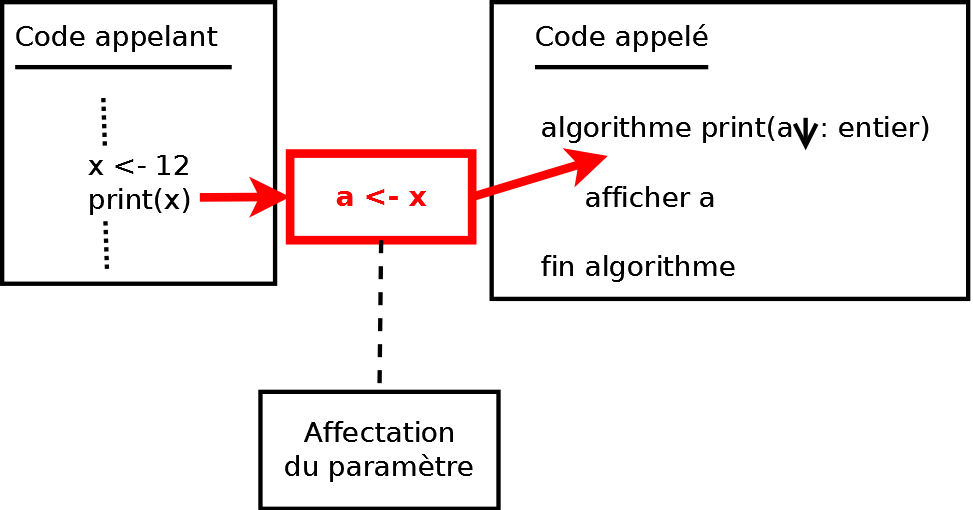
\includegraphics[width=0.8\textwidth]{image/figure-parametres-entrants}
        \caption{Paramètre entrant}
        \label{fig:gull}
    \end{subfigure}
\par\end{centering}

\vspace{1cm}

\begin{centering}
    \begin{subfigure}[b]{0.8\textwidth}
	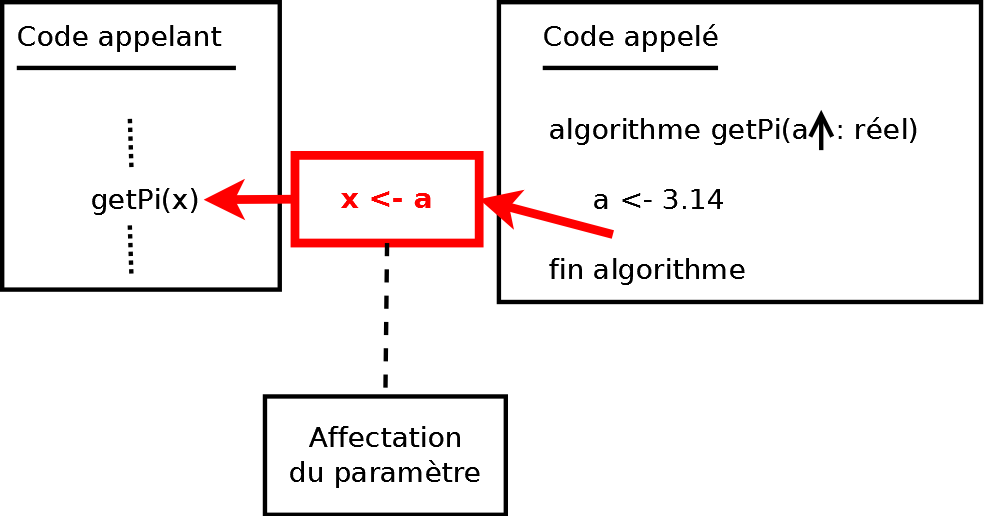
\includegraphics[width=0.8\textwidth]{image/figure-parametres-sortants}
        \caption{Paramètre sortant}
        \label{fig:gull}
    \end{subfigure}
\par\end{centering}

\vspace{1cm}

\begin{centering}
    \begin{subfigure}[b]{0.8\textwidth}
	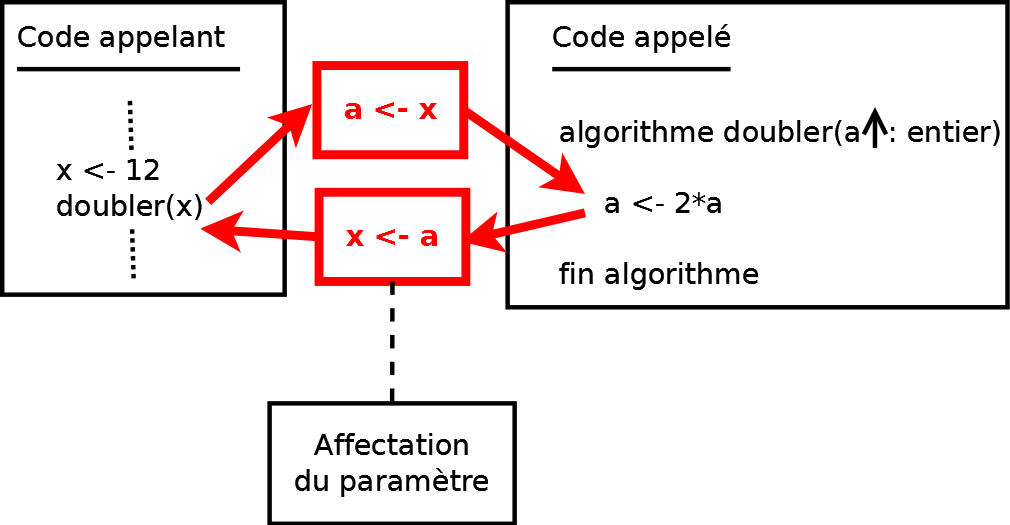
\includegraphics[width=0.8\textwidth]{image/figure-parametres-entrant-sortants}
        \caption{Paramètre entrant-sortant}
        \label{fig:gull}
    \end{subfigure}
\par\end{centering}

\protect\caption{\label{fig:parametres}Les trois types de paramètres}
\end{figure}
\end{center}

\clearpage{}


%===================
\section{Exercices}
%===================

	\begin{Exercice}{Tracer des algorithmes}
		Indiquer quels nombres sont successivement affichés 
		lors de l’exécution des algorithmes ex1, ex2, ex3 et ex4.
	
		\begin{LDA}
		\Algo{ex1}{}{}
			\Decl{x, y}{entiers}
			\Stmt addition(3, 4, x)
			\Write x
			\Let x \Gets 3
			\Let y \Gets 5
			\Stmt addition(x, y, y)
			\Write y
		\EndAlgo
		\Empty
		\Algo{addition}{a\In, b\In, c\Out~:~entiers}{}
			\Decl{somme}{entier}
			\Let somme \Gets a + b
			\Let c \Gets somme
		\EndAlgo
		\end{LDA}
	
		\begin{LDA}
		\Algo{ex2}{}{}
			\Decl{a, b}{entiers}
			\Stmt addition(3, 4, a) \Comment voir ci-dessus
			\Write a
			\Let a \Gets 3
			\Let b \Gets 5
			\Stmt addition(b, a, b)
			\Write b
		\EndAlgo
		\end{LDA}
	
		\begin{LDA}
		\Algo{ex3}{}{}
			\Decl{a, b, c}{entiers}
			\Stmt calcul(3, 4, c)
			\Write c
			\Let a \Gets 3
			\Let b \Gets 4
			\Let c \Gets 5
			\Stmt calcul(b, c, a)
			\Write a, b, c
		\EndAlgo
		\Empty
		\Algo{calcul}{a\In, b\In, c\Out~:~entiers}{}
			\Let a \Gets 2 * a
			\Let b \Gets 3 * b
			\Let c \Gets a + b
		\EndAlgo
		\end{LDA}
	
		\begin{LDA}
		\Algo{ex4}{}{}
			\Decl{a, b, c}{entiers}
			\Let a \Gets 3
			\Let b \Gets 4
			\Let c \Gets f(b)
			\Write c
			\Stmt calcul2(a, b, c)
			\Write a, b, c
		\EndAlgo
		\Empty
		\Algo{calcul2}{a\In, b\In, c\Out~:~entiers}{}
			\Let a \Gets f(a)
			\Let c \Gets 3 * b
			\Let c \Gets a + c
		\EndAlgo
		\Empty
		\Algo{f}{a\In~:~entier}{entier}
			\Decl{b}{entier}
			\Let b \Gets 2 * a + 1
			\Return b
		\EndAlgo
		\end{LDA}	
	\end{Exercice}
	
	\begin{Exercice}{Appels de module}
		Parmi les instructions suivantes (où les variables
		\lda{a}, \lda{b} et \lda{c}
		sont des entiers), lesquelles font correctement appel 
		à l’algorithme d’en-tête suivant~?
	
		\begin{LDA}
			\Entete{PGCD}{a\In,b\In~:~entiers}{entier}
		\end{LDA}
	
		\begin{LDA}
		\Stmt [1] a \Gets PGCD(24, 32)
		\Stmt [2] a \Gets PGCD(a, 24)
		\Stmt [3] b \Gets 3 * PGCD(a + b, 2*c) + 120
		\Stmt [4] PGCD(20, 30)
		\Stmt [5] a \Gets PGCD(a, b, c)
		\Stmt [6] a \Gets PGCD(a, b) + PGCD(a, c)
		\Stmt [7] a \Gets PGCD(a, PGCD(a, b))
		\Stmt [8] \Read PGCD(a, b)
		\Stmt [9] \Write PGCD(a, b)
		\Stmt [10] PGCD(a, b) \Gets c
		\end{LDA}
	\end{Exercice}
	
	\begin{Exercice}{Maximum de 4 nombres}
		Écrivez un algorithme qui calcule le maximum de 4 nombres.
	\end{Exercice}

	\begin{Exercice}{Écart entre 2 durées}
		Étant donné deux durées données chacune par trois
		nombres (heure, minute, seconde),
		écrire un algorithme qui calcule
		le délai écoulé entre ces deux durées en heure(s), minute(s),
		seconde(s) sachant que la deuxième durée donnée 
		est plus petite que la première.
	\end{Exercice}
	
	\begin{Exercice}{Réussir GEN1}
		Reprenons l’exercice \vref{algo:réussirGEN1}.
		Cette fois-ci on ne veut rien afficher
		mais fournir deux résultats~:
		un booléen indiquant si l’étudiant a réussi ou pas
		et un entier indiquant sa cote (qui n’a de sens que s’il a réussi). 
	\end{Exercice}

	\begin{Exercice}{Tirer une carte}
		L’exercice suivant a déjà été résolu. 
		Refaites une solution modulaire.
		
		Écrire un algorithme qui affiche l’intitulé d’une carte
		tirée au hasard dans un paquet de 52 cartes.
		Par exemple, "As de cœur", "3 de pique", "Valet de carreau"
		ou encore "Roi de trèfle".
	\end{Exercice}

	\begin{Exercice}{Nombre de jours dans un mois}
		Écrire un algorithme qui donne le nombre de jours dans un mois.
		Il reçoit en paramètre le numéro du mois (1 pour janvier\dots)
		ainsi que l’année.
		Pour le mois de février, 
		il faudra répondre 28 ou 29 selon que l’année fournie
		est bissextile ou pas.
		Vous devez réutiliser au maximum ce que vous avez déjà fait
		lors d’exercices précédents (cf. exercice \vref{ex:bissextile}).
	\end{Exercice}

	\begin{Exercice}{Valider une date}
		Écrire un algorithme qui valide 
		une date donnée par trois entiers~:~ l’année, le mois et le jour.
		Vous devez réutiliser au maximum ce que vous avez déjà fait
		lors d’exercices précédents.
	\end{Exercice}
	
	\begin{Exercice}{Généraliser un algorithme}
		Dans l’exercice \vref{algo:mult5},
		nous avons écrit un algorithme 
		pour tester si un nombre est divisible par 5.
		Si on vous demande à présent
		un algorithme pour tester si un nombre est divisible par 3,
		vous le feriez sans peine.
		Idem pour tester la divisibilité par 2, 4, 6, 7, 8, 9\dots{}
		mais vous vous lasseriez bien vite.
		
		N’est-il pas possible d’écrire un seul algorithme,
		plus général, qui résolve tous ces problèmes d’un coup~?  
	\end{Exercice}
	
